\documentclass[a4paper,11pt]{scrartcl}

\usepackage[utf8]{inputenc}
%\usepackage[ngerman]{babel}
\usepackage[T1]{fontenc}
\usepackage{amsmath}
\usepackage[left=3cm, right=2cm, top= 2cm, bottom = 2.5cm, includeheadfoot]{geometry}
\usepackage[svgnames]{xcolor}
%\usepackage{gnuplottex}
\usepackage{pdfpages}
\usepackage{listings} 
\lstset{
	basicstyle=\scriptsize\color{Black},
	keywordstyle=\color{SteelBlue}\bfseries,
	language = C,
	numbers=right, numberstyle=\tiny, stepnumber=5, numbersep=0pt,
	showstringspaces=false}
\usepackage{url}
\usepackage{setspace}
%umgebungen sind \begin(singlespace/onehalfspace/doublespace)
%einfacher eineinhalbfacher und 2facher zeilenabstand
%es kann aber auch nur mit {\singlespace bla bla} {\doublespace blabla } und {\onehalfspacing} gearbeitet werden.

\usepackage{times}
\usepackage{graphicx}
\usepackage{color}
\usepackage{fancyhdr}
\pagestyle{fancy}
\lhead{{\small Simon Stadlinger, Jonas Kordt}}
\chead{Übungsserie 4}
\rhead{{\small Programmiertechnik II}}

\rfoot{}
\cfoot{\thepage}
\lfoot{}

\usepackage{graphicx}

%\pagestyle{headings}

%Befehle um Kopfund Fuszeile Anzupassen:
%\thepage - Seitennummer
%\leftmark - Aktueller Kapitelname "Kapitel X. Name des Kapitels"
%\rightmark - Aktueller Untertitelname "X.X Name des Kapitels
%\chaptername - Das Wort "Kapitel"
%\thechapter - Aktuelle Kapitelnummerierung
%\thesection - Aktuelle Unterkapitelnummerierung
%\slshape - Kursiv und Sanseriv
\title{Übung XX}

\begin{document}
\begin{center}
\LARGE{\textbf{Aufgabe 1 - empirische Analyse}}
\end{center}
Für jeden Wert von N haben wir 10 Messungen durchgeführt (außer für Java - time N = 1000, da die Messungen hier sehr lange gedauert haben) und des Durchschnitt berechnet (siehe anhaenge/alle\_werte.xlsx). Mit dem Durchschnitt haben wir dann die Überprüfungen für O(N), O(N$^2$) und O(N$^3$) durchgeführt. 
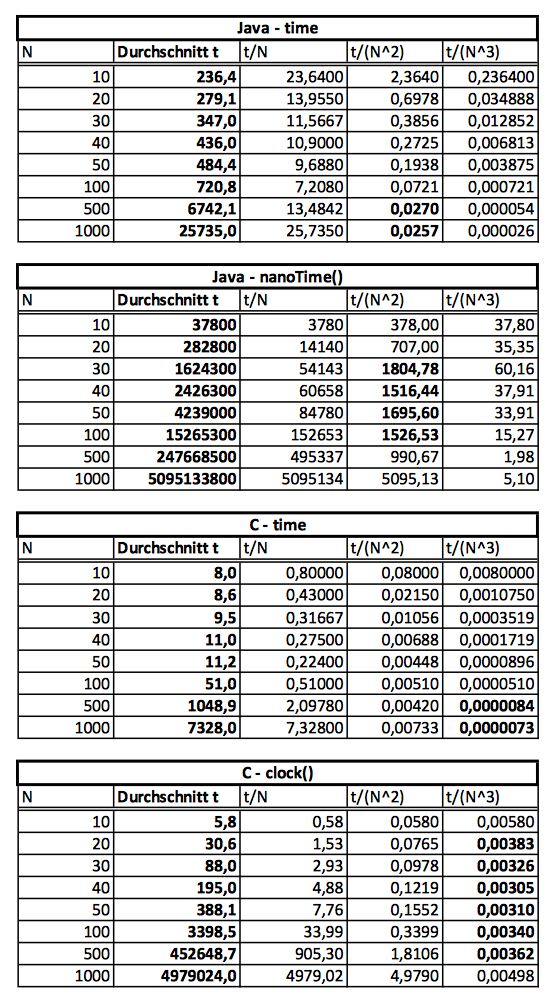
\includegraphics[width=.51\textwidth]{empirischer_test.png}\\
Java:\\
Die Gesamtlaufzeit (Java - time) ist stark von der Java Umgebung dominiert und daher sind die hohen Werte für N besonders relevant. Letztendlich kommen wir zu dem Ergebnis O(N$^2$)\\
Die Lauftzeit von mult (Java - nanoTime()) ist nicht mehr von Java Umgebung dominiert und die Werte sind erkennbar besser. Das Ergebnis O(N$^2$) ist hier deutlicher zu erkennen.\\\\
C:\\
Die Gesamtlaufzeit (C - time) ist von Faktoren wie der Initalisierung und Ausgabe beeinflusst weswegen die kubische Laufzeit erst bei großen N deutlich wird. Ergebnis: O(N$^3$).\\
Die Laufzeit von mult (C - clock()) ist nicht mehr von anderen faktoren beeinflusst und die kubische Laufzeit wird sehr deutliche. Ergebnis: O(N$^3$).





\end{document}
